\documentclass[11pt,reqno]{amsart}

\usepackage[T1]{fontenc}
\usepackage{lmodern}
\usepackage[letterpaper,margin=1in]{geometry}
\usepackage{amsmath,amssymb,amsthm,mathtools}
\usepackage{graphicx}
\usepackage{booktabs,array}
\usepackage{xcolor}
\usepackage{microtype}
\usepackage[numbers,sort&compress]{natbib}
\usepackage{hyperref}

% Unified Three-Role Semantic Palette (matching Figures 1--8):
%   colW: Workers (W)               -- Cobalt Blue
%   colF: Frontier Orchestrator (F) -- Royal Crimson-Plum
%   colH: Human Overseer (H)        -- Forest Emerald-Teal
\definecolor{colW}{RGB}{25,100,186}
\definecolor{colF}{RGB}{157,23,77}
\definecolor{colH}{RGB}{15,118,94}
\definecolor{linkink}{RGB}{30,58,95}
\definecolor{warn}{RGB}{204,82,14}

\hypersetup{
  colorlinks=true,
  linkcolor=linkink,
  citecolor=linkink,
  urlcolor=linkink,
  breaklinks=true
}

\linespread{1.05}
\setlength{\parskip}{3.6pt plus 1.2pt minus 0.5pt}
\setlength{\parindent}{0pt}
\setlength{\abovedisplayskip}{8pt plus 2pt minus 2pt}
\setlength{\belowdisplayskip}{8pt plus 2pt minus 2pt}
\setlength{\floatsep}{9pt plus 2pt minus 2pt}
\setlength{\textfloatsep}{10pt plus 2pt minus 2pt}
\setlength{\intextsep}{9pt plus 2pt minus 2pt}
\setlength{\jot}{6.5pt}
\renewcommand{\topfraction}{0.90}
\renewcommand{\bottomfraction}{0.88}
\renewcommand{\textfraction}{0.08}
\renewcommand{\floatpagefraction}{0.82}
\allowdisplaybreaks[2]

\newtheoremstyle{spacious}%
  {10pt plus 3pt minus 2pt}%
  {10pt plus 3pt minus 2pt}%
  {\itshape}%
  {}%
  {\bfseries}%
  {.}%
  {0.5em}%
  {}
\theoremstyle{spacious}
\newtheorem{proposition}{Proposition}[section]

% Semantic role macros for prose and mathematical variables
\newcommand{\Wtxt}[1]{\textcolor{colW}{#1}}
\newcommand{\Ftxt}[1]{\textcolor{colF}{#1}}
\newcommand{\Htxt}[1]{\textcolor{colH}{#1}}
\newcommand{\Wv}[1]{{\color{colW}#1}}
\newcommand{\Fv}[1]{{\color{colF}#1}}
\newcommand{\Hv}[1]{{\color{colH}#1}}

\newcommand{\E}{\mathbb{E}}
\newcommand{\Prob}{\mathbb{P}}
\newcommand{\ask}{\mathtt{ask}}
\newcommand{\play}{\mathtt{play}}
\newcommand{\oversee}{{\color{colH}\mathtt{oversee}}}
\newcommand{\trust}{{\color{colH}\mathtt{trust}}}
\newcommand{\Over}{{\color{colH}\mathrm{Over}}}

\title[Who Gets to Ask for Help?]{Who Gets to Ask for Help?\\Coordinating \texorpdfstring{\Htxt{Human}}{Human} Oversight in Agent Swarms}

\author{Jiayuan Sheng}
\address{Columbia University, New York, NY 10027}
\email{js6646@columbia.edu}

\author{Mohamed El Amine Lakhnichi}
\address{Columbia University, New York, NY 10027}
\email{ml5000@columbia.edu}
\date{November 26, 2026 \quad $\cdot$ \quad Project Proposal for DROM B9157: \emph{Algorithms for Social Systems: Beyond i.i.d.\ Environments}}

\begin{document}

\begin{abstract}
Agentic workflows increasingly pair a high-stakes \Ftxt{Frontier Orchestrator} with many parallel low-cost \Wtxt{Workers} under a single capacity-constrained \Htxt{Human Overseer}. While single-agent oversight protocols align deferral with \Htxt{human} welfare and classical queueing suggests serving high-stakes requests first, shared \Htxt{human} congestion breaks both intuitions in a two-tier swarm. Even truthful \Wtxt{worker} deferrals with zero false alarms crowd out \Ftxt{orchestrator} oversight past a critical swarm size, and small priority-classification errors or mild \Htxt{reviewer} alarm fatigue re-trigger \Ftxt{orchestrator} collapse along sharp crossover scaling laws. Resolving this congestion externality requires coordinating identical \Wtxt{workers} before deferrals reach the inbox: a fixed-size rotating roster strictly outperforms both unrestricted deferral and total \Wtxt{worker} silence, and independent policy-gradient learners break symmetry into a small active \Wtxt{worker} cohort and silent peers.
\end{abstract}

\maketitle

\section{Introduction}
\label{sec:intro}

Agentic AI deployments increasingly organize computation as a \emph{two-tier swarm} in which one capable \Ftxt{Frontier Orchestrator} ($\Fv{F}$) coordinates $N$ parallel low-cost \Wtxt{Workers} ($\Wv{W_1},\dots,\Wv{W_N}$)~\cite{anthropic2025research,kimi2026k25}. Current designs sit at two extremes: orchestrator--worker products prevent \Wtxt{workers} from reaching the user directly, whereas AI-control monitoring pipelines and open research swarms allow every parallel instance to escalate to a shared \Htxt{human} audit channel~\cite{greenblatt2024control,lindner2025control,paglieri2026swarm}. We study the regime between these extremes when all agents share one \Htxt{Human Overseer} ($\Hv{H}$)~\cite{wang2026ask,lindner2025control}. In the two-player \emph{Oversight Game} of \href{https://arxiv.org/abs/2510.26752}{Overman and Bayati}~\cite{overman2026oversight}, wrapping an immutable pretrained base policy in a $\{\play,\ask\}\times\{\trust,\oversee\}$ interface turns autonomy calibration into a cooperative Markov Potential Game, leaving the multi-agent shared-\Htxt{reviewer} extension open~\cite{overman2026oversight,turan2026capacity}. Without capacity limits, multi-agent off-switch games show that individual corrigibility composes when rewards are additive and can fail otherwise~\cite{agrawal2026offswitch}.

Shared \Htxt{human} attention breaks this compositionality even when every agent maximizes the exact same additive team reward. Because all $N$ \Wtxt{workers} and the \Ftxt{orchestrator} defer into one \Htxt{human} inbox, cautious \Wtxt{worker} deferrals impose a congestion externality~\cite{lykouris2024congested,saketos2026defer} that crowds out high-stakes \Ftxt{orchestrator} oversight. Moreover, whereas classical queueing protects high-priority traffic via strict priority service~\cite{argon2009priority,ouyang2022priorities} and multi-agent clarification controllers rely on centralized scheduling~\cite{wang2026ask,costen2024shared}, small priority misclassification rates~\cite{argon2009priority} or mild clutter-induced \Htxt{reviewer} fatigue~\cite{turan2026capacity,zhang2026falcon} re-ignite \Ftxt{orchestrator} crowding out along closed-form scaling laws. Preventing collapse requires \emph{admission coordination among identical \Wtxt{workers}} before deferrals enter the inbox: a zero-training fixed-size rotating roster strictly beats both unrestricted deferral and complete \Wtxt{worker} silence, and decentralized independent policy-gradient (IPG) learners with independent per-\Wtxt{worker} parameters sort into deterministic active askers and silent peers matching that optimal roster.

\textbf{Organization.} \hyperref[sec:formulation]{Section~\ref{sec:formulation}} formulates the two-tier Oversight Game, \Htxt{human} attention models, and deferral policies; \hyperref[sec:experiments]{Section~\ref{sec:experiments}} presents the main crowding-out and admission-coordination results; and \hyperref[sec:conclusion]{Section~\ref{sec:conclusion}} discusses strategic deployment implications. Proofs, priority-noise and fatigue experiments, and extended literature positioning appear in \hyperref[app:proofs]{Appendices~\ref{app:proofs}}--\hyperref[app:extra]{\ref{app:extra}}.

\section{Model Formulation}
\label{sec:formulation}

Following~\cite{overman2026oversight}, we hold the pretrained base policies of both tiers fixed and study how \Wtxt{worker} admission policies and \Htxt{human} capacity govern safety and oversight cost (\hyperref[fig:architecture]{Figure~\ref{fig:architecture}}).

\begin{figure}[!htbp]
  \centering
  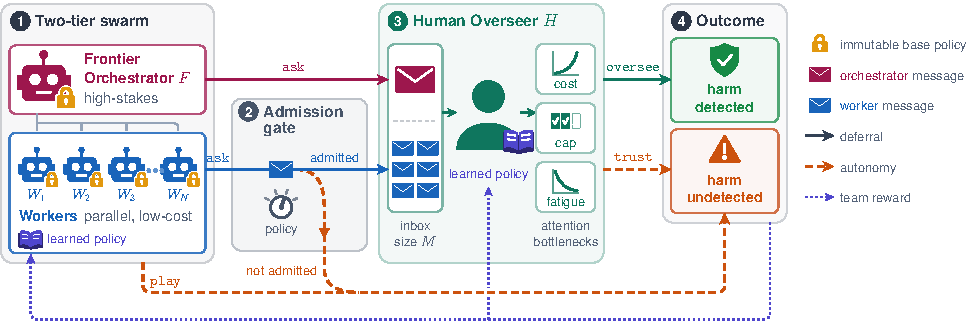
\includegraphics[width=\linewidth]{fig_architecture.pdf}
  \caption{Two-tier Oversight Game pipeline. Deferred queries (\emph{pings}) from \Wtxt{Workers} ($\Wv{W_1},\dots,\Wv{W_N}$) pass an admission gate (\hyperref[fig:policies]{Figure~\ref{fig:policies}}), whereas the \Ftxt{orchestrator} ($\Fv{F}$) defers directly into the \Htxt{Human Overseer}'s ($\Hv{H}$) shared inbox of size $M$. $\Over$ eliminates harm only under $(\ask,\oversee)$; under $\play$ or $(\ask,\trust)$ the base action executes autonomously.}
  \label{fig:architecture}
\end{figure}

\subsection*{Two-Tier Swarm and Oversight Interface}
Each episode comprises $N$ exchangeable \emph{\Wtxt{Workers}} ($i = 1,\dots,N$) with immutable base policies $\Wv{\sigma_i}$, one high-stakes \emph{\Ftxt{orchestrator}} ($\Fv{F}$) with immutable base policy $\Fv{\sigma_F}$, and one \emph{\Htxt{Human Overseer}} ($\Hv{H}$). Every AI agent chooses from $\mathcal{A}_{\mathrm{AI}} = \{\play,\ask\}$ and $\Hv{H}$ responds to each deferred ping with an action from $\Hv{\mathcal{A}_{\mathrm{H}}} = \{\trust,\oversee\}$~\cite{overman2026oversight}. Tier $t \in \{\Wv{W}, \Fv{F}\}$ independently encounters a risky state with probability $p_t \in (0,1)$, incurring harm $L_t > 0$ if executed unreviewed ($\Fv{L_F} \gg \Wv{L_W}$). Choosing $\ask$ with recall $h_t = \Prob(\ask\mid\text{risky})$ and false-alarm rate $q_t = \Prob(\ask\mid\text{safe})$ generates $\Wv{A_i} \sim \mathrm{Bernoulli}(\Wv{r_W})$ and $\Fv{A_F} \sim \mathrm{Bernoulli}(\Fv{r_F})$ with marginal deferral rate $r_t := p_t h_t + (1 - p_t) q_t$. $\Over$ eliminates an agent's harm under $(\ask,\oversee)$ and executes its base action otherwise. $\Hv{H}$ observes a shared inbox of size
\[
  M \;=\; \Fv{A_F} + \Wv{W}, \qquad \Wv{W} \;:=\; \sum_{i=1}^N \Wv{A_i} \;\sim\; \mathrm{Binomial}(N, \Wv{r_W}),
\]
where overseeing one deferred ping from tier $t \in \{\Wv{W}, \Fv{F}\}$ averts posterior expected harm
\[
  B_t \;:=\; \frac{p_t h_t}{r_t}\,L_t, \qquad \Fv{B_F} \;\gg\; \Wv{B_W}.
\]

\subsection*{\Htxt{Human} Attention Models}
We evaluate three stylized \Htxt{human} supervision bottlenecks~\cite{lykouris2024congested,lindner2025control,turan2026capacity}:
\begin{enumerate}
  \setlength{\itemsep}{2pt}
  \item \textbf{Cost:} Reviewing a ping in an inbox of size $m$ incurs convex cost $\Hv{c}(m) = \Hv{c_0} m^{\Hv{\gamma}}$ ($\Hv{c_0} > 0, \Hv{\gamma} > 1$)~\cite{lykouris2024congested,saketos2026defer}. Rational $\Hv{H}$ plays $\oversee$ on tier $t$ iff $B_t \ge \Hv{c}(m)$, yielding cutoffs $m_t := \lfloor (B_t / \Hv{c_0})^{1/\Hv{\gamma}} \rfloor$ with $\Fv{m_F} > \Wv{m_W}$.
  \item \textbf{Cap:} $\Hv{H}$ reviews at most $\Hv{K} \ge 1$ pings per episode~\cite{greenblatt2024control,lindner2025control,alves2024deccaf}. $\Fv{F}$ pings are labeled high priority while \Wtxt{worker} pings are misclassified as high priority with probability $\Hv{\varepsilon} \in [0,1]$~\cite{argon2009priority}, with uniform tie-breaking ($\Hv{\varepsilon}=0$: \Ftxt{orchestrator}-first; $\Hv{\varepsilon}=1$: random triage).
  \item \textbf{Fatigue:} $\Hv{H}$ reviews all pings in priority order at flat cost $\Hv{c_0} < \Wv{B_W}$, but clutter degrades accuracy~\cite{turan2026capacity,zhang2026falcon} so $\Over$ neutralizes risk with probability $\Hv{\xi}(m) = e^{-\Hv{\lambda}(m-1)}$ ($\Hv{\lambda} \ge 0$).
\end{enumerate}

\subsection*{Deferral and Admission Policies}
We compare four \Wtxt{worker} policies (\hyperref[fig:policies]{Figure~\ref{fig:policies}}); $\Fv{F}$ always defers directly. \textbf{Policy~1} keeps all \Wtxt{workers} at base rates $(\Wv{h_W}, \Wv{q_W})$; \textbf{Policy~2} sets $\Wv{W} \equiv 0$, either absorbing \Wtxt{worker} risk (\textbf{2a}) or applying an automated \Ftxt{orchestrator} filter with detection rate $\Fv{d_F} \in (0,1)$ (\textbf{2b}). Our \textbf{fixed-size rotating roster} uniformly permits $j \in \{0,\dots,N\}$ \Wtxt{workers} to $\ask$ each episode, replacing $\mathrm{Binomial}(N, \Wv{r_W})$ by $\mathrm{Binomial}(j, \Wv{r_W})$ without training. \textbf{Policy~3} casts the swarm as a cooperative Markov Potential Game~\cite{overman2026oversight}: each \Wtxt{Worker} $i$ updates softmax $\ask$ rates $(\Wv{h_i}, \Wv{q_i})$ and $\Hv{H}$ updates $\oversee$ probabilities $\Hv{\pi_{\mathrm{H}}}(t, m)$ via independent policy gradient (IPG) on shared team reward $R_\Phi = -\E[\mathrm{Harm}] - \E[\mathrm{Cost}]$.

\begin{figure}[!htbp]
  \centering
  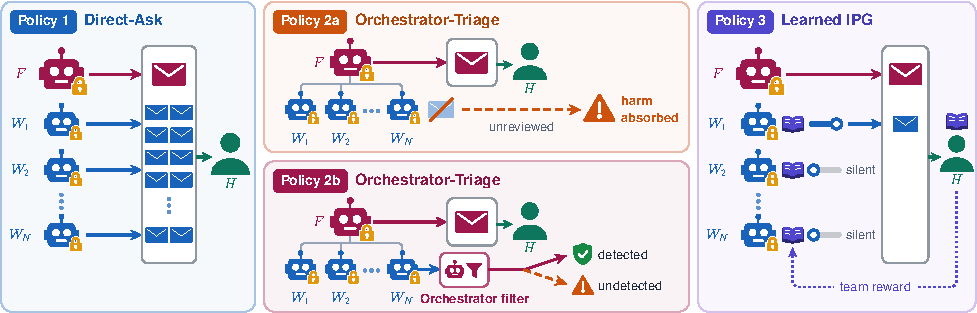
\includegraphics[width=\linewidth]{fig_policies.pdf}
  \caption{\Wtxt{Worker} deferral under Policy~1 (left), Policies~2a/2b (middle), and Policy~3 (right; books mark learned policies, sliders each \Wtxt{worker}'s learned $\ask$ rate). The fixed-size rotating roster interpolates between Policy~1 ($j = N$) and Policy~2a ($j = 0$).}
  \label{fig:policies}
\end{figure}

\section{Experimental Results}
\label{sec:experiments}

We evaluate exact Binomial expectations corroborated by Monte Carlo simulation; baseline calibration and IPG specifications appear in \hyperref[subsec:calibration]{Appendix~\ref{subsec:calibration}} and formal proofs in \hyperref[app:proofs]{Appendix~\ref{app:proofs}}.

\subsection{Zero-False-Alarm \texorpdfstring{\Wtxt{Worker}}{Worker} Deferral Crowds Out \texorpdfstring{\Ftxt{Orchestrator}}{Orchestrator} Oversight}
\label{subsec:crowding}

In a single-agent Oversight Game, raising true-positive deferral recall at zero false alarms ($\Wv{q_W} = 0$) monotonically lowers harm. \hyperref[fig:crowding]{Figure~\ref{fig:crowding}} shows that shared \Htxt{human} congestion reverses this property in two stages as swarm size $N$ grows. Under the cost bottleneck, cautious \Wtxt{worker} pings first push inbox volume past the \Wtxt{worker} cutoff $\Wv{m_W}$ (\emph{\Wtxt{worker}-on-\Wtxt{worker} crowding out}) and then past $\Fv{m_F}$ as well, collapsing conditional \Ftxt{orchestrator} oversight (\hyperref[prop:crowding]{Proposition~\ref{prop:crowding}}) while causing observed \Htxt{human} reviews to plummet as $\Hv{H}$ defaults to $\trust$ (\hyperref[subsec:review_volume]{Appendix~\ref{subsec:review_volume}}). Under the cap bottleneck ($\Hv{K}=2$, random triage), \Ftxt{orchestrator} dilution starts immediately and false alarms ($\Wv{q_W}>0$) accelerate collapse across both regimes. Consequently, \textbf{Policy~1} excels only at small $N$ and low $\Wv{q_W}$; \textbf{Policy~2b} achieves the lowest harm across scales when an accurate \Ftxt{orchestrator} filter ($\Fv{d_F}$) exists, while \textbf{Policy~2a} overtakes Policy~1 past $N^*$; and \textbf{Policy~3} matches Policy~1 at small $N$ while throttling \Wtxt{worker} pings to preserve \Ftxt{orchestrator} oversight without an automated filter. Moreover, \hyperref[subsec:scaling_roster]{Appendix~\ref{subsec:scaling_roster}} shows that strict \Ftxt{orchestrator}-first priority queues do not rescue Policy~1 once priority labels carry slight noise ($\Hv{\varepsilon} > 0$, where $N^* \propto 1/(\Wv{r_W}\Hv{\varepsilon})$ by \hyperref[prop:noisy_priority]{Proposition~\ref{prop:noisy_priority}}) or inbox clutter induces mild \Htxt{reviewer} fatigue ($\Hv{\lambda} > 0$, where $N^* \sim \log(1/\Hv{\lambda})/(\Wv{r_W}\Hv{\lambda})$ by \hyperref[prop:roster]{Proposition~\ref{prop:roster}}).

\begin{figure}[!htbp]
  \centering
  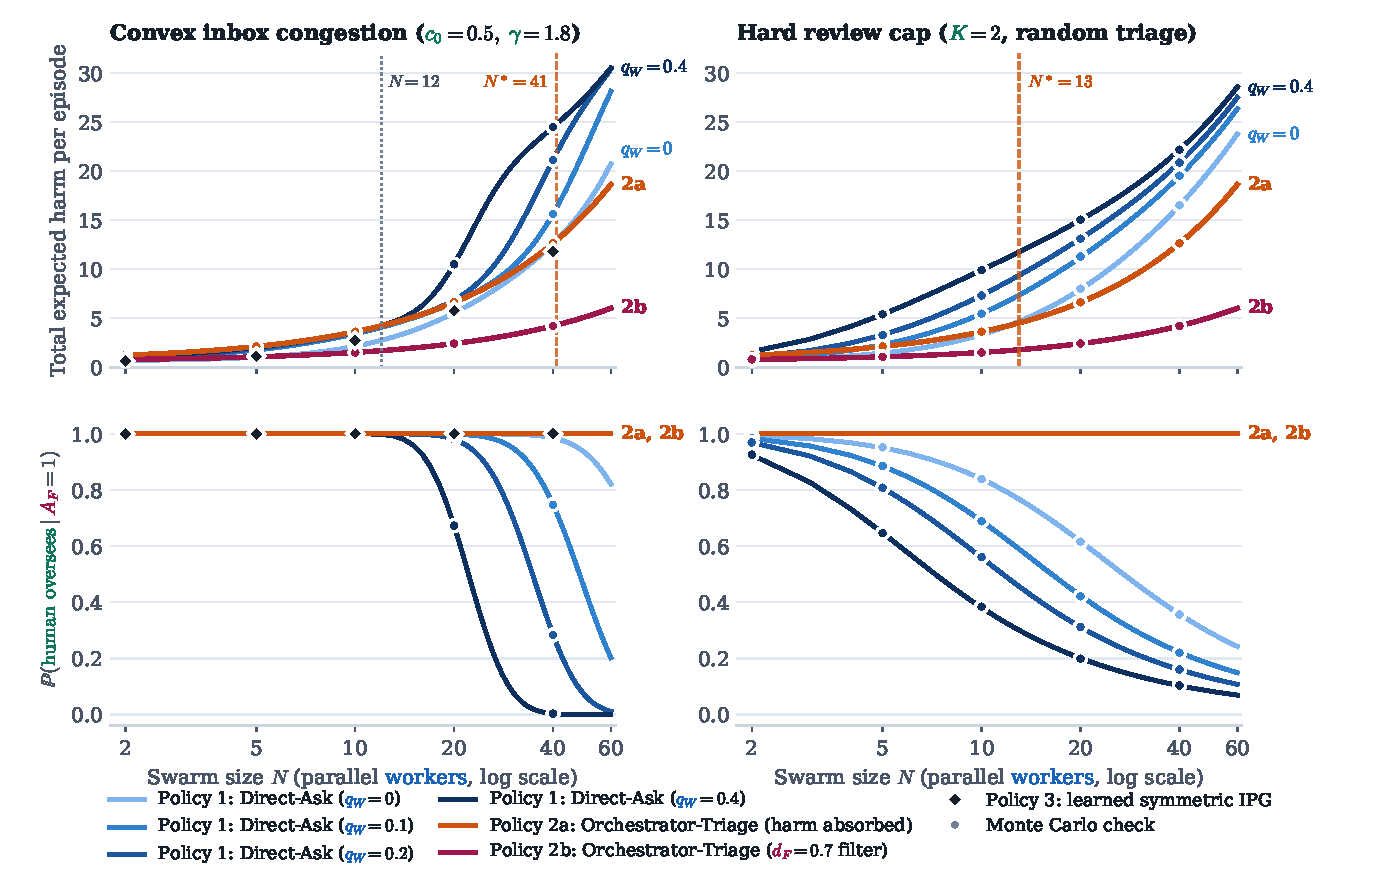
\includegraphics[width=0.94\linewidth]{fig_crowding_vs_N.pdf}
  \caption{Total expected harm (top) and conditional \Ftxt{orchestrator} oversight probability $\Prob(\Hv{H}\text{ oversees}\mid \Fv{A_F}=1)$ (bottom) versus swarm size $N$ under convex inbox congestion (left) and hard cap $\Hv{K}=2$ with random triage (right).}
  \label{fig:crowding}
\end{figure}

\subsection{Admission Coordination via Rotating Rosters and Decentralized IPG}
\label{subsec:specialization}

When automated \Ftxt{orchestrator} filtering is unavailable, safe scaling requires restricting \Wtxt{worker} admissions before pings enter the inbox. \hyperref[prop:roster]{Proposition~\ref{prop:roster}} and \hyperref[subsec:scaling_roster]{Appendix~\ref{subsec:scaling_roster}} show that our zero-training \textbf{fixed-size rotating roster} traces a strictly U-shaped harm curve across $j \in \{0,\dots,N\}$, achieving an interior optimum $0 < j^* \ll N$ that beats both unrestricted escalation ($j=N$) and total \Wtxt{worker} silence ($j=0$). \hyperref[fig:specialization]{Figure~\ref{fig:specialization}} tests whether decentralized IPG learners (\textbf{Policy~3}) discover this coordination without a central controller under the cost bottleneck (sensitivity to permissive initial \Htxt{human} trust appears in \hyperref[subsec:trust_trap]{Appendix~\ref{subsec:trust_trap}}). Across all $N$, IPG eliminates \Wtxt{worker} false alarms and throttles aggregate pings below the \Htxt{human}'s cutoff to preserve \Ftxt{orchestrator} review. Crucially, when identical \Wtxt{workers} maintain independent logits under sampled $N$-player IPG rather than a single shared policy, they do not remain at uniform throttling: at $N = 40$, they sort into a small cohort of deterministic active askers ($\Wv{h_i} \approx 1$) and silent peers ($\Wv{h_i} \approx 0$), matching the team-loss-optimal rotating roster. \hyperref[prop:symbreak]{Proposition~\ref{prop:symbreak}} explains this convergence: because expected team welfare is multilinear in independent \Wtxt{worker} admission rates, every interior symmetric optimum is a saddle point (cf.~\cite{emmons2022symmetric}) dominated by a binary roster of size $j^*$ that reduces inbox variance relative to uniform thinning~\cite{hoeffding1956successes}, paralleling reinforcement-learning sorting in market-entry games~\cite{duffy2005sorting,whitehead2008elfarol} within a cooperative oversight game with a co-learning \Htxt{human}.

\begin{figure}[!htbp]
  \centering
  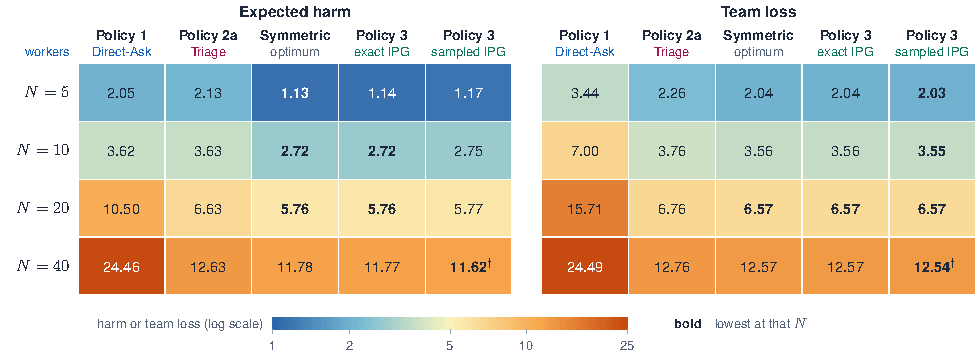
\includegraphics[width=0.98\linewidth]{fig_specialization.pdf}
  \caption{Expected harm (left) and team loss (right) by swarm size $N$ and policy under convex inbox congestion (Policy~1 at $\Wv{q_W} = 0.4$; Policy~3 initialized at $\Wv{q_{W,0}} = 0.4, \Hv{p_{H,0}} = 0.5$). Colour encodes one shared logarithmic scale; bold marks each row's minimum. $^\dagger$Midpoint over the four of five seeds electing four active \Wtxt{worker} askers (harm $11.60$--$11.63$, team loss $12.52$--$12.55$; fifth seed elects three askers at harm $11.80$, \hyperref[subsec:calibration]{Appendix~\ref{subsec:calibration}}).}
  \label{fig:specialization}
\end{figure}

\section{Conclusion}
\label{sec:conclusion}

Scaling single-agent oversight to a swarm reveals two counter-intuitive failure modes. First, uncoordinated \Wtxt{worker} caution can lower safety: even zero-false-alarm \Wtxt{worker} deferrals crowd out high-stakes \Ftxt{orchestrator} review and push a congested \Htxt{human} into passive auto-approval, making falling intervention rates mask rising harm. Second, inbox prioritization is fragile at scale---slight priority-label noise or mild \Htxt{reviewer} fatigue re-triggers \Ftxt{orchestrator} collapse---whereas admission control succeeds by breaking symmetry among identical \Wtxt{workers} into a small active cohort and silent peers. Strategically, these findings explain why production orchestrator--worker systems insulate users from direct subagent interrupts and cap subagent fan-out by query complexity~\cite{anthropic2025research}. Instead of routing parallel escalations synchronously to one \Htxt{human}, deployments should reserve blocking \Htxt{human} review for irreversible \Ftxt{orchestrator} commits while governing \Wtxt{worker} trajectories via automated \Ftxt{orchestrator} filtering~\cite{anthropic2025research}, asynchronous post-hoc auditing~\cite{lindner2025control}, or---when weight-sharing subagents require live \Htxt{human} spot-checks---a rotating admission roster.

\clearpage
\begingroup
\setlength{\parskip}{1.2pt}
\setlength{\bibsep}{0pt}
\raggedright
\sloppy
\begin{thebibliography}{99}

\bibitem{agrawal2026offswitch}
A.~Agrawal, S.~Ebadian, and L.~Hammond (2026). The multi-agent off-switch game. In \emph{Proceedings of the 25th International Conference on Autonomous Agents and Multiagent Systems (AAMAS 2026)}; \href{https://openreview.net/pdf?id=XXW1dIcgik}{openreview.net/pdf?id=XXW1dIcgik}.

\bibitem{alves2024deccaf}
J.~V.~Alves, D.~Leit\~ao, S.~Jesus, M.~O.~P.~Sampaio, J.~Li\'ebana, P.~Saleiro, M.~A.~T.~Figueiredo, and P.~Bizarro (2024). Cost-sensitive learning to defer to multiple experts with workload constraints. \emph{Transactions on Machine Learning Research (TMLR)}; \href{https://arxiv.org/abs/2403.06906}{arXiv:2403.06906}.

\bibitem{amir2026diversity}
M.~Amir, M.~Bettini, and A.~Prorok (2026). When is diversity rewarded in cooperative multi-agent learning? In \emph{International Conference on Learning Representations (ICLR 2026)}; \href{https://arxiv.org/abs/2506.09434}{arXiv:2506.09434}.

\bibitem{ancker2017alertfatigue}
J.~S.~Ancker, A.~Edwards, S.~Nosal, D.~Hauser, E.~Mauer, and R.~Kaushal (2017). Effects of workload, work complexity, and repeated alerts on alert fatigue in a clinical decision support system. \emph{BMC Medical Informatics and Decision Making}, 17(1):36. \href{https://pmc.ncbi.nlm.nih.gov/articles/PMC5387195/}{pmc.ncbi.nlm.nih.gov/articles/PMC5387195}.

\bibitem{anthropic2025research}
Anthropic (2025). \emph{How we built our multi-agent research system}. \href{https://www.anthropic.com/research/multi-agent-research-system}{anthropic.com/research/multi-agent-research-system}.

\bibitem{anthropic2026autonomy}
Anthropic (2026). \emph{Measuring AI agent autonomy in practice}. \href{https://www.anthropic.com/research/measuring-agent-autonomy}{anthropic.com/research/measuring-agent-autonomy}.

\bibitem{anthropic2026multiagent}
Anthropic (2026). \emph{Patterns and problems in emerging multiagent systems}. \href{https://www.anthropic.com/research/multiagent-systems}{anthropic.com/research/multiagent-systems}.

\bibitem{argon2009priority}
N.~T.~Argon and S.~Ziya (2009). Priority assignment under imperfect information on customer type identities. \emph{Manufacturing \& Service Operations Management}, 11(4):674--693. \href{https://pubsonline.informs.org/doi/10.1287/msom.1080.0246}{doi:10.1287/msom.1080.0246}.

\bibitem{casheekar2026report}
A.~M.~Casheekar and H.~Tangirala (2026). \emph{Learning to report unsafe tasks in a multi-agent game}. \href{https://arxiv.org/abs/2610.09002}{arXiv:2610.09002}.

\bibitem{chien2012queues}
S.-Y.~Chien, H.~Wang, and M.~Lewis (2012). Human vs.\ algorithmic scheduling for multi-robot supervision. In \emph{Proceedings of the Human Factors and Ergonomics Society Annual Meeting}.

\bibitem{costen2024shared}
C.~Costen, A.~Gautier, N.~Hawes, and B.~Lacerda (2024). Multi-robot allocation of assistance from a shared uncertain operator. In \emph{Proceedings of the 23rd International Conference on Autonomous Agents and Multiagent Systems (AAMAS 2024)}, pp.~400--408. \href{https://www.ifaamas.org/Proceedings/aamas2024/pdfs/p400.pdf}{ifaamas.org/Proceedings/aamas2024/pdfs/p400.pdf}.

\bibitem{dahiya2022restless}
A.~Dahiya, N.~Akbarzadeh, A.~Mahajan, and S.~L.~Smith (2021/2022). \emph{Scalable operator allocation for multi-robot assistance: A restless bandit approach}. \href{https://arxiv.org/abs/2111.06437}{arXiv:2111.06437}.

\bibitem{duffy2005sorting}
J.~Duffy and E.~Hopkins (2005). Learning, information, and sorting in market entry games: Theory and evidence. \emph{Games and Economic Behavior}, 51(1):31--62. \href{https://ideas.repec.org/a/eee/gamebe/v51y2005i1p31-62.html}{repec:eee:gamebe:v51y2005i1p31-62}.

\bibitem{emmons2022symmetric}
S.~Emmons, C.~Oesterheld, A.~Critch, V.~Conitzer, and S.~Russell (2022). For learning in symmetric teams, local optima are global Nash equilibria. In \emph{International Conference on Machine Learning (ICML 2022)}, PMLR 162:5924--5943; \href{https://arxiv.org/abs/2207.03470}{arXiv:2207.03470}.

\bibitem{greenblatt2024control}
R.~Greenblatt, B.~Shlegeris, K.~Sachan, and F.~Roger (2024). AI control: Improving safety despite intentional subversion. In \emph{International Conference on Machine Learning (ICML 2024)}, PMLR 235:16295--16336; \href{https://arxiv.org/abs/2312.06942}{arXiv:2312.06942}.

\bibitem{hoeffding1956successes}
W.~Hoeffding (1956). On the distribution of the number of successes in independent trials. \emph{Annals of Mathematical Statistics}, 27(3):713--721. \href{https://projecteuclid.org/journals/annals-math-stat/1177728178}{doi:10.1214/aoms/1177728178}.

\bibitem{hoque2023fleet}
R.~Hoque, L.~Y.~Chen, S.~Sharma, K.~Dharmarajan, B.~Thananjeyan, P.~Abbeel, and K.~Goldberg (2023). Fleet-DAgger: Interactive robot fleet learning with scalable human supervision. In \emph{Conference on Robot Learning (CoRL)}, PMLR 205. \href{https://proceedings.mlr.press/v205/hoque23a.html}{proceedings.mlr.press/v205/hoque23a.html}.

\bibitem{kimi2026k25}
Kimi Team / Moonshot AI (2026). \emph{Kimi K2.5: Visual Agentic Intelligence}. \href{https://arxiv.org/abs/2602.02276}{arXiv:2602.02276}.

\bibitem{moonshot2026k25blog}
Moonshot AI (2026). \emph{Kimi K2.5 Tech Blog: Visual Agentic Intelligence}. \href{https://www.kimi.ai/blog/kimi-k2-5}{kimi.ai/blog/kimi-k2-5}.

\bibitem{kleinberg2009multiplicative}
R.~Kleinberg, G.~Piliouras, and \'E.~Tardos (2009). Multiplicative updates outperform generic no-regret learning in congestion games. In \emph{Proceedings of the 41st Annual ACM Symposium on Theory of Computing (STOC 2009)}, pp.~533--542. \href{https://www.cs.cornell.edu/~rdk/papers/stoc09.pdf}{cs.cornell.edu/\~{}rdk/papers/stoc09.pdf}.

\bibitem{lindner2025control}
D.~Lindner, C.~Griffin, T.~Korbak, R.~S.~Zimmermann, G.~Irving, S.~Farquhar, and A.~Cooney (2025). \emph{Practical challenges of control monitoring in frontier AI deployments}. \href{https://arxiv.org/abs/2512.22154}{arXiv:2512.22154}.

\bibitem{lykouris2024congested}
T.~Lykouris and W.~Weng (2024/2025). \emph{Learning to defer in congested systems: The AI-human interplay}. \href{https://arxiv.org/abs/2402.12237}{arXiv:2402.12237}.

\bibitem{marschak1972teams}
J.~Marschak and R.~Radner (1972). \emph{Economic Theory of Teams}. Yale University Press, New Haven, CT.

\bibitem{mclaughlin2024complementarity}
B.~McLaughlin and J.~Spiess (2024). \emph{Designing algorithmic recommendations to achieve human--AI complementarity}. \href{https://arxiv.org/abs/2405.01484}{arXiv:2405.01484}.

\bibitem{olsen2004fanout}
D.~R.~Olsen Jr.\ and S.~B.~Wood (2004). Fan-out: Measuring human control of multiple robots. In \emph{Proceedings of the SIGCHI Conference on Human Factors in Computing Systems (CHI 2004)}, pp.~231--238.

\bibitem{openai2025agents}
OpenAI (2025). \emph{New tools for building agents (Agents SDK)}. \href{https://openai.com/index/new-tools-for-building-agents/}{openai.com/index/new-tools-for-building-agents}.

\bibitem{ouyang2022priorities}
H.~Ouyang, N.~T.~Argon, and S.~Ziya (2022). Assigning priorities (or not) in service systems with nonlinear waiting costs. \emph{Management Science}, 68(2):1233--1255. \href{https://pubsonline.informs.org/doi/10.1287/mnsc.2020.3952}{doi:10.1287/mnsc.2020.3952}.

\bibitem{overman2026oversight}
W.~Overman and M.~Bayati (2025/2026). \emph{The Oversight Game: Learning to cooperatively balance an AI agent's safety and autonomy}. ICML 2026; \href{https://arxiv.org/abs/2510.26752}{arXiv:2510.26752}.

\bibitem{overman2026conservatism}
W.~Overman and M.~Bayati (2026). \emph{Calibrating conservatism for scalable oversight}. ICML 2026; \href{https://arxiv.org/abs/2605.28807}{arXiv:2605.28807}.

\bibitem{paglieri2026swarm}
D.~Paglieri, L.~Cross, T.~Genewein, J.~Z.~Leibo, N.~Tomasev, and A.~S.~Vezhnevets (2026). \emph{A case study on emergent cheating and whistleblowing in autonomous research swarms}. \href{https://arxiv.org/abs/2609.04170}{arXiv:2609.04170} (companion essay by D.~Paglieri and A.~S.~Vezhnevets, \href{https://institute.deepmind.com/essays/cheaters-and-whistleblowers-in-the-agent-swarm/}{institute.deepmind.com/essays/cheaters-and-whistleblowers-in-the-agent-swarm}).

\bibitem{reid2026risks}
A.~Reid, S.~O'Callaghan, D.~Venini, L.~Carroll, and T.~Caetano (2026). \emph{Risks and controls for multi-agent systems: An analytical framework for deployment of AI agents across organisational boundaries}. Australian AI Safety Institute; \href{https://arxiv.org/abs/2608.26626}{arXiv:2608.26626}.

\bibitem{ruan2024toolemu}
Y.~Ruan, H.~Dong, A.~Wang, S.~Pitis, Y.~Zhou, J.~Ba, Y.~Dubois, C.~J.~Maddison, and T.~Hashimoto (2024). Identifying the risks of LM agents with an LM-emulated sandbox. In \emph{International Conference on Learning Representations (ICLR 2024)}; \href{https://arxiv.org/abs/2309.15817}{arXiv:2309.15817}.

\bibitem{saketos2026defer}
V.~Saketos, W.~Reveillard, A.~Proutiere, S.~Dalleiger, and M.~Xiao (2026). \emph{To defer or not to defer? Online learning with LLMs and congested experts}. \href{https://arxiv.org/abs/2610.15128}{arXiv:2610.15128}.

\bibitem{tong2026contextual}
Y.~Tong (2026). \emph{A contextual-bandit oversight game with two-sided informational asymmetry}. \href{https://arxiv.org/abs/2607.00155}{arXiv:2607.00155}.

\bibitem{turan2026capacity}
E.~Turan (2026). \emph{Oversight has a capacity: Calibrating agent guards to a subjective, fatiguing human}. \href{https://arxiv.org/abs/2606.08919}{arXiv:2606.08919}.

\bibitem{wang2026ask}
H.~Wang, S.~Liu, and Z.~Wang (2026). \emph{When should AI agents ask? Clarification requests under limited human attention}. \href{https://arxiv.org/abs/2610.41129}{arXiv:2610.41129}.

\enlargethispage{1.2\baselineskip}
\bibitem{whitehead2008elfarol}
D.~Whitehead (2008). \emph{The El Farol bar problem revisited: Reinforcement learning in a potential game}. Edinburgh School of Economics Discussion Paper 186. \href{https://ideas.repec.org/p/edn/esedps/186.html}{repec:edn:esedps:186}.

\bibitem{zhang2026falcon}
Z.~Zhang, C.~C.~Nguyen, D.~Rosewarne, K.~Wells, and G.~Carneiro (2026). \emph{Fatigue-aware learning to defer via constrained optimisation}. \href{https://arxiv.org/abs/2604.00904}{arXiv:2604.00904}.

\end{thebibliography}
\endgroup

\clearpage
\appendix

\section{Formal Propositions and Proofs}
\label{app:proofs}

Throughout this appendix, let $\Wv{W} = \sum_{i=1}^N \Wv{A_i} \sim \mathrm{Binomial}(N, \Wv{r_W})$ denote the \Wtxt{worker} deferral count, independent of $\Fv{A_F} \sim \mathrm{Bernoulli}(\Fv{r_F})$ with $\Fv{a} := \Fv{r_F}$, and let $M = \Wv{W} + \Fv{A_F}$ denote total inbox size observed by $\Hv{H}$.

\begin{proposition}[Sharp Capacity Boundary and Crowding-Out Threshold]
\label{prop:crowding}
Fix $\Wv{r_W} > 0$, $\Fv{p_F h_F} > 0$, and $\Fv{B_F} > \Wv{B_W}$.
\begin{enumerate}
  \setlength{\itemsep}{4pt}
  \item[(i)] Under hard-cap random triage ($\Hv{K} \ge 1$) with zero \Wtxt{worker} false alarms ($\Wv{q_W} = 0$), silencing \Wtxt{workers} (\textbf{Policy~2a}) achieves strictly lower expected harm than Direct-Ask (\textbf{Policy~1}) for all sufficiently large $N$ \emph{if and only if} $\Fv{p_F h_F L_F} > \Hv{K} \Wv{L_W}$. When $\Fv{p_F h_F L_F} \le \Hv{K} \Wv{L_W}$, Policy~1 remains weakly safer at every $N \ge 1$.
  \item[(ii)] Under convex inbox congestion ($\Hv{c_0} > 0, \Hv{\gamma} > 1$) with $\Fv{B_F} > \Hv{c}(1)$, even at $\Wv{q_W} = 0$, there exists a finite threshold $N^*$ such that $\E[\mathrm{Harm}(\mathrm{P2a})] < \E[\mathrm{Harm}(\mathrm{P1})]$ for all $N \ge N^*$.
\end{enumerate}
\end{proposition}

\begin{proof}
The idea is to compare expected harm averted under Policy~1 and Policy~2a by separating \Wtxt{worker}-tier oversight gains from \Ftxt{orchestrator} crowding-out losses. Under Policy~2a, $M = \Fv{A_F} \in \{0,1\}$, so $\Hv{H}$ always oversees $\Fv{F}$ whenever $\Fv{A_F} = 1$ (since $\Hv{K} \ge 1$ and $\Fv{B_F} > \Hv{c}(1)$), averting expected harm $\Fv{a B_F} = \Fv{p_F h_F L_F}$.

\medskip
\noindent\textbf{(i) Hard review cap $\Hv{K}$, uniform random triage ($\Wv{q_W} = 0$).}
Condition on the realized \Wtxt{worker} ping count $\Wv{W} = \Wv{w}$ and average over $\Fv{A_F} \sim \mathrm{Bernoulli}(\Fv{a})$:
\begin{itemize}
  \setlength{\itemsep}{3pt}
  \item When $\Wv{w} < \Hv{K}$, every ping in the inbox is reviewed by $\Hv{H}$, averting expected harm $\Wv{w B_W} + \Fv{a B_F}$.
  \item When $\Wv{w} \ge \Hv{K}$, exactly $\Hv{K}$ pings are reviewed; conditional on $\Fv{A_F} = 1$, the \Ftxt{orchestrator} ping is selected with probability $\Hv{K} / (\Wv{w} + 1)$, averting expected harm
  \[
    \Hv{K} \Wv{B_W} + \Fv{a} (\Fv{B_F} - \Wv{B_W})\,\frac{\Hv{K}}{\Wv{w} + 1}.
  \]
\end{itemize}
As $N \to \infty$, $\Prob(\Wv{W} \ge \Hv{K}) \to 1$ and $\E[\Hv{K} / (\Wv{W} + 1)] \to 0$, so expected harm averted under Policy~1 converges to
\[
  \lim_{N \to \infty} \E\big[\mathrm{Averted}(\mathrm{P1})\big] \;=\; \Hv{K} \Wv{B_W} \;=\; \Hv{K} \Wv{L_W},
\]
whereas Policy~2a averts $\Fv{p_F h_F L_F}$. Hence Policy~2a strictly dominates at large $N$ if and only if $\Fv{p_F h_F L_F} > \Hv{K} \Wv{L_W}$, whereas $\Fv{a B_F} \le \Hv{K} \Wv{B_W}$ makes Policy~1 weakly safer at every $N \ge 1$.

\medskip
\noindent\textbf{(ii) Convex inbox congestion ($\Hv{c_0} > 0, \Hv{\gamma} > 1, \Fv{B_F} > \Hv{c}(1)$).}
Observing inbox size $m$, $\Hv{H}$ oversees tier $t \in \{\Wv{W}, \Fv{F}\}$ iff $m \le m_t := \lfloor (B_t / \Hv{c_0})^{1/\Hv{\gamma}} \rfloor$. Defining coverage probabilities $\Fv{\rho_F}(N) := \Prob(\Wv{W} \le \Fv{m_F} - 1)$ and $\Wv{\rho_W}(N) := \Prob(\Fv{A_F} + \Wv{W_{-1}} \le \Wv{m_W} - 1)$, expected harm satisfies
\begin{align*}
  \E\big[\mathrm{Harm}(\mathrm{P1})\big] - \E\big[\mathrm{Harm}(\mathrm{P2a})\big]
  &\;=\; \underbrace{\Fv{p_F h_F L_F} \big(1 - \Fv{\rho_F}(N)\big)}_{\text{\Ftxt{Orchestrator} crowding-out loss}}
     \;-\; \underbrace{N\,\Wv{p_W h_W L_W}\,\Wv{\rho_W}(N)}_{\text{\Wtxt{Worker} oversight gain}}.
\end{align*}
Because $\E[\Wv{W}] = N \Wv{r_W} \to \infty$, Chernoff's bound gives $\Fv{\rho_F}(N) \to 0$ and $0 \le N \Wv{p_W h_W L_W}\Wv{\rho_W}(N) \le \Wv{m_W L_W}\Prob(\Wv{W} \le \Wv{m_W}) \to 0$, so the difference converges to $\Fv{p_F h_F L_F} > 0$.
\end{proof}

\begin{proposition}[Imperfect Priority Scaling Law]
\label{prop:noisy_priority}
Suppose every \Ftxt{orchestrator} ping is assigned high priority, each received \Wtxt{worker} ping is independently misclassified as high priority with probability $\Hv{\varepsilon_N} \in [0,1]$, and high-priority ties are broken uniformly by $\Hv{H}$ under cap $\Hv{K} \ge 1$. With $\Wv{T} \sim \mathrm{Binomial}(N, \Wv{r_W} \Hv{\varepsilon_N})$, conditional \Ftxt{orchestrator} coverage equals
\[
  \Fv{\rho_F}(N) \;=\; \E\!\left[\min\!\left(1,\, \frac{\Hv{K}}{1 + \Wv{T}}\right)\right].
\]
At $\Hv{\varepsilon_N} = 0$, $\Wv{T} \equiv 0$ and $\Fv{\rho_F}(N) \equiv 1$ (so Policy~1 weakly dominates Policy~2a at every $N$), whereas for any fixed $\Hv{\varepsilon_N} \equiv \Hv{\varepsilon} > 0$, $\Fv{\rho_F}(N) \to 0$ as $N \to \infty$. In the Poisson regime $N \Wv{r_W} \Hv{\varepsilon_N} \to x > 0$ with $\Hv{K} = 2$, coverage converges to $\Fv{\rho_F}(x) = \frac{2(1 - e^{-x})}{x} - e^{-x}$, crossing below the Policy~2a break-even coverage $\Fv{\rho_F^*} = \frac{\Fv{a B_F} - \Hv{K} \Wv{B_W}}{\Fv{a}(\Fv{B_F} - \Wv{B_W})}$ at a unique $x^* > 0$ and yielding $N^* \sim x^*/(\Wv{r_W} \Hv{\varepsilon})$.
\end{proposition}

\begin{proof}
The idea is to price any work-conserving triage rule $\pi$ under cap $\Hv{K}$ solely through its conditional \Ftxt{orchestrator} coverage $\Fv{\rho_F}(\pi)$. Writing $\Hv{V_N} := \E[\min(\Hv{K}, M)]$ for expected total reviews performed by $\Hv{H}$, every reviewed \Wtxt{worker} ping averts $\Wv{B_W}$ whereas reviewing $\Fv{F}$ in place of a \Wtxt{worker} averts an additional $\Fv{B_F} - \Wv{B_W} > 0$:
\begin{align*}
  \E\big[\mathrm{Harm}(\pi)\big]
  &\;=\; \E\big[\mathrm{Harm}_{\mathrm{unreviewed}}\big]
     \;-\; \underbrace{\Wv{B_W} \Hv{V_N}}_{\text{Baseline slot value}}
     \;-\; \underbrace{\Fv{a} (\Fv{B_F} - \Wv{B_W})\,\Fv{\rho_F}(\pi)}_{\text{\Ftxt{Orchestrator} priority premium}}.
\end{align*}
Conditional on $\Fv{A_F} = 1$ and $\Wv{T}$ misclassified \Wtxt{worker} pings, uniform tie-breaking among the $1 + \Wv{T}$ high-priority pings selects $\Fv{F}$ with probability $\min(1, \Hv{K}/(1+\Wv{T}))$, which equals $1$ at $\Hv{\varepsilon}=0$ and vanishes as $N \to \infty$ for any fixed $\Hv{\varepsilon} > 0$. In the Poisson limit $\Wv{T} \Rightarrow \mathrm{Poisson}(x)$ at $\Hv{K} = 2$,
\begin{align*}
  \Fv{\rho_F}(x)
  &\;=\; e^{-x} + x e^{-x} + \sum_{k=2}^\infty \frac{2}{k + 1}\,\frac{x^k e^{-x}}{k!}
   \;=\; \frac{2(1 - e^{-x})}{x} - e^{-x}.
\end{align*}
Equating $\E[\mathrm{Harm}(\pi)] = \E[\mathrm{Harm}(\mathrm{P2a})]$ yields $\Fv{\rho_F^*} = (\Fv{a B_F} - \Wv{B_W} \Hv{V_N}) / [\Fv{a}(\Fv{B_F} - \Wv{B_W})]$, and since $\Hv{V_N} \to \Hv{K} = 2$ and $\Fv{\rho_F}(x)$ strictly decreases from $1$ to $0$, solving $\Fv{\rho_F}(x^*) = \Fv{\rho_F^*}$ uniquely determines $x^*$ and $N^* \sim x^*/(\Wv{r_W}\Hv{\varepsilon})$.
\end{proof}

\begin{proposition}[Optimal Fixed-Size Rotating Roster and Fatigue Silence Boundary]
\label{prop:roster}
Let $j \in \{0,\dots,N\}$ denote the fixed number of \Wtxt{workers} permitted to $\ask$ per episode.
\begin{enumerate}
  \setlength{\itemsep}{4pt}
  \item[(i)] Under hard cap $\Hv{K} \ge 2$ with arbitrary misclassification probability $\Hv{\varepsilon} \in [0,1]$, permitting $j = 1$ \Wtxt{worker} guarantees $M \le 2 \le \Hv{K}$, strictly lowering expected harm by $\Wv{p_W h_W L_W} > 0$ relative to total silence ($j = 0$). Hence total \Wtxt{worker} silence is never optimal among roster policies.
  \item[(ii)] Under flat per-review cost $\Hv{c_0} < \Wv{B_W}$ with exponential alarm fatigue $\Hv{\xi}(m) = e^{-\Hv{\lambda}(m-1)}$, let $\Fv{A} := \Fv{p_F h_F L_F}$, $\Wv{C} := \Wv{p_W h_W L_W}$, $\Hv{\eta} := 1 - e^{-\Hv{\lambda}}$, and $d := 1 - \Wv{r_W} \Hv{\eta}$. Expected harm averted by roster size $j$ equals
  \[
    S(j) \;=\; \Fv{A} d^j + \Wv{C} j (1 - \Fv{a}\Hv{\eta}) d^{j-1}.
  \]
  Consequently, $S(j)$ is unimodal on $\{0,\dots,N\}$, total \Wtxt{worker} silence ($j^* = 0$) minimizes harm if and only if $\Hv{\eta} (\Fv{A} \Wv{r_W} + \Fv{a} \Wv{C}) \ge \Wv{C}$, and the unrestricted-versus-silence crossover $S(N) = \Fv{A}$ scales as
  \[
    N^* \;\sim\; \frac{\log(1/\Hv{\lambda})}{\Wv{r_W} \Hv{\lambda}} \qquad (\Hv{\lambda} \to 0).
  \]
\end{enumerate}
\end{proposition}

\begin{proof}
The idea is to evaluate exact binomial moment generating functions over the permitted \Wtxt{worker} ping count $\Wv{W_j} \sim \mathrm{Binomial}(j, \Wv{r_W})$. Part~(i) follows immediately from $M = \Fv{A_F} + \Wv{A_1} \le 2 \le \Hv{K}$ at $j=1$. For part~(ii), conditioning on $\Wv{W_j}$ gives $\E[e^{-\Hv{\lambda} \Wv{W_j}}] = (1 - \Wv{r_W}\Hv{\eta})^j = d^j$ on $\Fv{F}$ and $\E[e^{-\Hv{\lambda}(\Fv{A_F} + \Wv{W_{j-1}})}] = (1 - \Fv{a}\Hv{\eta}) d^{j-1}$ on each permitted \Wtxt{worker}, yielding $S(j) = d^{j-1}[\Fv{A} d + \Wv{C}(1 - \Fv{a}\Hv{\eta}) j]$. Because $S(j+1) - S(j)$ changes sign at most once from positive to negative, $S(j)$ is unimodal and $j^* = 0$ is optimal iff $S(1) \le S(0)$, i.e., $\Hv{\eta}(\Fv{A} \Wv{r_W} + \Fv{a} \Wv{C}) \ge \Wv{C}$. Equating $S(N) = \Fv{A}$ gives $d^{-N} = 1 + \frac{\Wv{C}(1 - \Fv{a}\Hv{\eta})}{\Fv{A} d} N$, so $-\log d \sim \Wv{r_W}\Hv{\lambda}$ yields $N^* \Wv{r_W}\Hv{\lambda} \sim \log(1/\Hv{\lambda})$.
\end{proof}

\begin{proposition}[Multilinear Symmetry Breaking and Roster Optimality]
\label{prop:symbreak}
Let $U(\Wv{u_1},\dots,\Wv{u_N})$ denote expected team welfare when each \Wtxt{Worker} $i$ independently receives admission permission with probability $\Wv{u_i} \in [0,1]$, and set $f(\Wv{u}) := U(\Wv{u},\dots,\Wv{u})$.
\begin{enumerate}
  \setlength{\itemsep}{4pt}
  \item[(i)] At any interior symmetric critical point $\Wv{u^*} \in (0,1)$ with $f'(\Wv{u^*}) = 0$ and $f''(\Wv{u^*}) < 0$, every unilateral \Wtxt{worker} deviation has zero first-order effect, whereas shifting two \Wtxt{workers} to $\Wv{u^*} + \delta$ and $\Wv{u^*} - \delta$ strictly increases team welfare by
  \[
    U(\Wv{u^*} + \delta,\, \Wv{u^*} - \delta,\, \Wv{u^*},\dots,\Wv{u^*}) - f(\Wv{u^*})
    \;=\; -\,\frac{f''(\Wv{u^*})}{N(N - 1)}\,\delta^2 \;>\; 0.
  \]
  \item[(ii)] Globally over $[0,1]^N$, team welfare attains its maximum at a deterministic binary corner $\Wv{\mathbf{u}^*} \in \{0,1\}^N$ corresponding to a fixed-size active \Wtxt{worker} roster of size $j^* = \sum_{i=1}^N \Wv{u_i^*}$:
  \[
    \max_{\Wv{\mathbf{u}} \in [0,1]^N} U(\Wv{\mathbf{u}})
    \;=\; \max_{j \in \{0,\dots,N\}} U(\mathbf{1}_j, \mathbf{0}_{N-j}).
  \]
\end{enumerate}
\end{proposition}

\begin{proof}
The idea is to exploit multilinearity of $U(\Wv{u_1},\dots,\Wv{u_N})$ in the independent Bernoulli permission indicators $\Wv{I_i} \sim \mathrm{Bernoulli}(\Wv{u_i})$: conditioning on $\Wv{I_i}$ shows that $U$ is affine in each $\Wv{u_i}$ separately ($\partial_{ii}^2 U \equiv 0$). By exchangeability along the diagonal $\Wv{\mathbf{u}} = (\Wv{u},\dots,\Wv{u})$,
\[
  f'(\Wv{u}) \;=\; N\,\partial_1 U(\Wv{\mathbf{u}}), \qquad
  f''(\Wv{u}) \;=\; N(N - 1)\,\partial_{12}^2 U(\Wv{\mathbf{u}}).
\]
At $\Wv{u^*}$ with $f'(\Wv{u^*}) = 0$ and $f''(\Wv{u^*}) < 0$, multilinearity in $(\Wv{u_1}, \Wv{u_2})$ makes the second-order expansion exact:
\[
  U(\Wv{u^*} + \delta,\, \Wv{u^*} - \delta,\, \Wv{u^*},\dots,\Wv{u^*}) - f(\Wv{u^*})
  \;=\; -\,\delta^2\,\partial_{12}^2 U(\Wv{\mathbf{u}^*})
  \;=\; -\,\frac{f''(\Wv{u^*})}{N(N - 1)}\,\delta^2 \;>\; 0.
\]
For part~(ii), coordinate-wise maximization of an affine function on $[0,1]$ replaces each fractional $\Wv{u_i} \in (0,1)$ with an endpoint in $\{0,1\}$ without decreasing $U$; by \Wtxt{worker} symmetry, every vertex depends only on $j = \sum_{i=1}^N \Wv{u_i}$.
\end{proof}

\section{Calibration and Supplementary Experimental Results}
\label{app:details}

\subsection{Baseline Calibration and Policy~3 Training Specifications}
\label{subsec:calibration}

All experiments evaluate the baseline two-tier calibration:
\[
  \Wv{p_W} = 0.15,\quad \Wv{L_W} = 2,\quad \Fv{p_F} = 0.25,\quad \Fv{L_F} = 50,\quad \Wv{h_W} = 0.90,\quad \Fv{h_F} = 0.95,\quad \Fv{q_F} = 0.05,
\]
with \Htxt{human} parameters $\Hv{c_0} = 0.5$, $\Hv{\gamma} = 1.8$, hard cap $\Hv{K} = 2$, and \Ftxt{orchestrator} filter detection rate $\Fv{d_F} = 0.70$ (giving convex-cost cutoffs $\Wv{m_W} = 2$ and $\Fv{m_F} = 11$ at $\Wv{q_W} = 0$, and crowding out under hard cap whenever $\Hv{K} \le 5$ since $\Fv{p_F h_F L_F} = 11.875 > \Hv{K}\Wv{L_W}$). In \hyperref[fig:specialization]{Figure~\ref{fig:specialization}}, Policy~3 is initialized from $\Hv{p_{H,0}} = 0.5$ and $\Wv{q_{W,0}} = 0.4$: exact symmetric IPG runs $40{,}000$ steps (learning rate $0.5$, step clip $1.0$, converging to $\Wv{q} \approx 0$ and $\Wv{h} \approx 3.5/N$), while sampled $N$-player REINFORCE runs $6{,}000$ steps (batch $2{,}048$, learning rate $0.3$) for $N \le 20$ and $30{,}000$ steps (batch $1{,}024$, learning rate $0.5$, $5$ seeds conditioned on the \Ftxt{orchestrator} cell for variance reduction) at $N = 40$.

\subsection{Priority-Noise and Alarm-Fatigue Scaling Laws and Rotating Rosters}
\label{subsec:scaling_roster}

A natural queueing remedy for \hyperref[subsec:crowding]{Subsection~\ref{subsec:crowding}} is to assign strict priority to \Ftxt{orchestrator} pings and decouple review effort from unreviewed queue length. While noiseless \Ftxt{orchestrator}-first triage ($\Hv{\varepsilon} = 0, \Hv{\lambda} = 0$) keeps conditional \Ftxt{orchestrator} coverage at $1.0$ for all $N$, \hyperref[fig:scaling]{Figure~\ref{fig:scaling}} shows that this idealized benchmark is knife-edge fragile. Under hard cap $\Hv{K} = 2$ (\hyperref[fig:scaling]{Figure~\ref{fig:scaling}}A), misclassifying even a small fraction $\Hv{\varepsilon} > 0$ of \Wtxt{worker} pings as high priority~\cite{argon2009priority} builds a competing high-priority backlog that drives \Ftxt{orchestrator} coverage toward zero along the inverse-error scaling law $N^* \sim x^*/(\Wv{r_W}\Hv{\varepsilon})$ (\hyperref[prop:noisy_priority]{Proposition~\ref{prop:noisy_priority}}). Independently, under flat per-review cost in strict \Ftxt{orchestrator}-first order (\hyperref[fig:scaling]{Figure~\ref{fig:scaling}}B), mild clutter-induced fatigue ($\Hv{\lambda} > 0$) degrades error-catching accuracy on the \Ftxt{orchestrator} step along $N^* \sim \log(1/\Hv{\lambda})/(\Wv{r_W}\Hv{\lambda})$, reaching a regime where silencing all \Wtxt{workers} is optimal even at $N = 1$ (\hyperref[prop:roster]{Proposition~\ref{prop:roster}(ii)}).

\begin{figure}[!htbp]
  \centering
  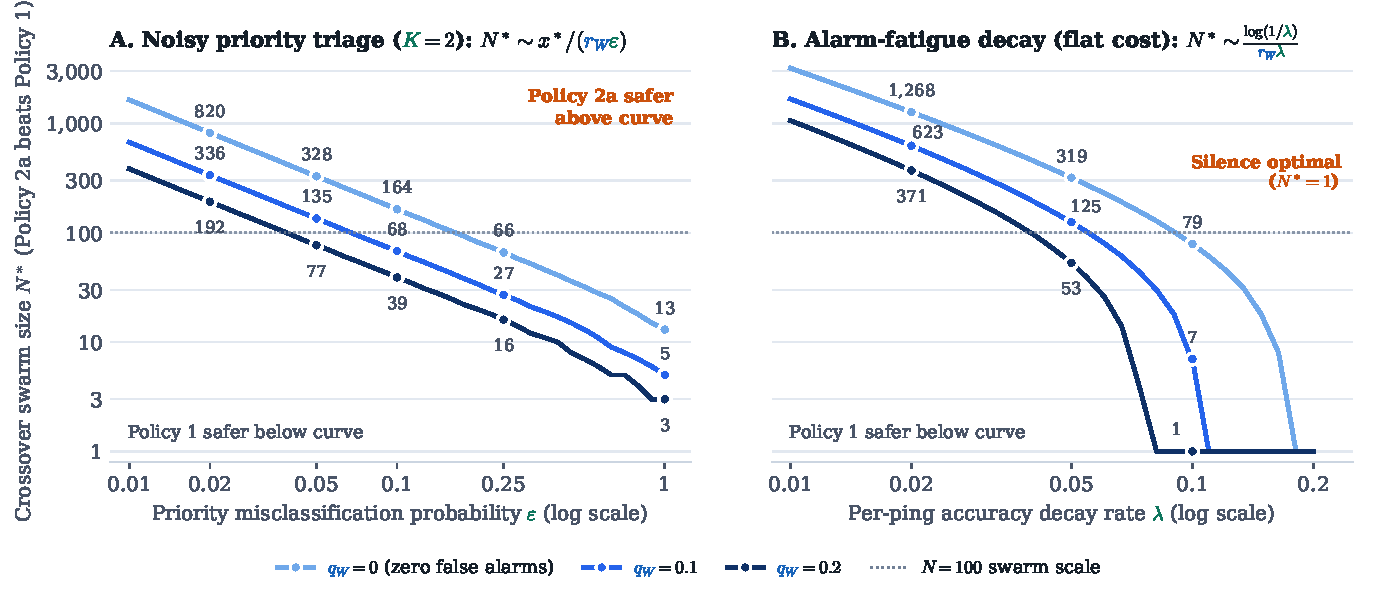
\includegraphics[width=0.94\linewidth]{fig_scaling_laws.pdf}
  \caption{Critical swarm-size thresholds $N^*$ above which silencing \Wtxt{workers} (Policy~2a) beats Direct-Ask (Policy~1) on log--log axes under (A) hard cap $\Hv{K}=2$ with noisy priority ($\Hv{\varepsilon}$) and (B) flat-cost alarm fatigue ($\Hv{\lambda}$).}
  \label{fig:scaling}
\end{figure}

Whenever neither automated \Ftxt{orchestrator} filtering (Policy~2b) nor multi-agent IPG training (Policy~3) is available in these noisy-priority or fatiguing regimes, \hyperref[fig:roster]{Figure~\ref{fig:roster}} demonstrates how our zero-training \textbf{fixed-size rotating roster} restores safe scaling past $N^*$ ($N = 80, \Wv{q_W} = 0$). Unrestricted escalation ($j = 80$, Policy~1) floods or fatigues \Ftxt{orchestrator} supervision worse than silencing all \Wtxt{workers} ($j = 0$, Policy~2a), whereas complete silence leaves spare \Htxt{human} review capacity unused; expected harm is strictly U-shaped in $j$, attaining an interior optimum $0 < j^* \ll N$ under both bottlenecks (\hyperref[prop:roster]{Proposition~\ref{prop:roster}}) while preserving ex-ante symmetry across \Wtxt{workers} via uniform episode-by-episode rotation.

\begin{figure}[!htbp]
  \centering
  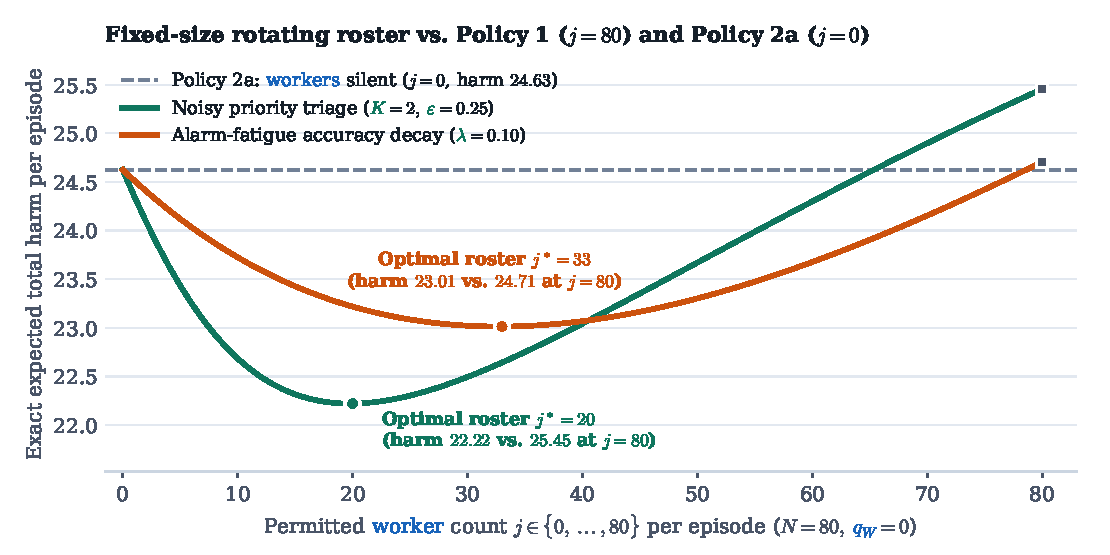
\includegraphics[width=0.80\linewidth]{fig_optimal_roster.pdf}
  \caption{Exact expected harm across permitted \Wtxt{worker} counts $j \in \{0,\dots,80\}$ under noisy priority ($\Hv{K}=2, \Hv{\varepsilon}=0.25$) and alarm fatigue ($\Hv{\lambda}=0.10$) at $N = 80, \Wv{q_W} = 0$, illustrating the interior U-shaped optimum $0 < j^* < N$.}
  \label{fig:roster}
\end{figure}

\subsection{Non-Monotonic Review Volume Under Passive Loss of Control}
\label{subsec:review_volume}

\hyperref[fig:review_volume]{Figure~\ref{fig:review_volume}} diagnoses \emph{passive loss of control}~\cite{overman2026oversight} under convex inbox congestion: expected \Htxt{human} reviews per episode are strongly non-monotonic in $N$, peaking at moderate swarm size and dropping below the \Wtxt{worker}-silent Policy~2a baseline at large $N$ or elevated $\Wv{q_W}$ precisely because congestion drives $\Hv{H}$ to play $\trust$ on nearly every query. Low observed \Htxt{human} intervention rates in deployment logs~\cite{anthropic2026autonomy} therefore cannot be read as safe autonomy without conditioning on unreviewed queue volume.

\begin{figure}[!htbp]
  \centering
  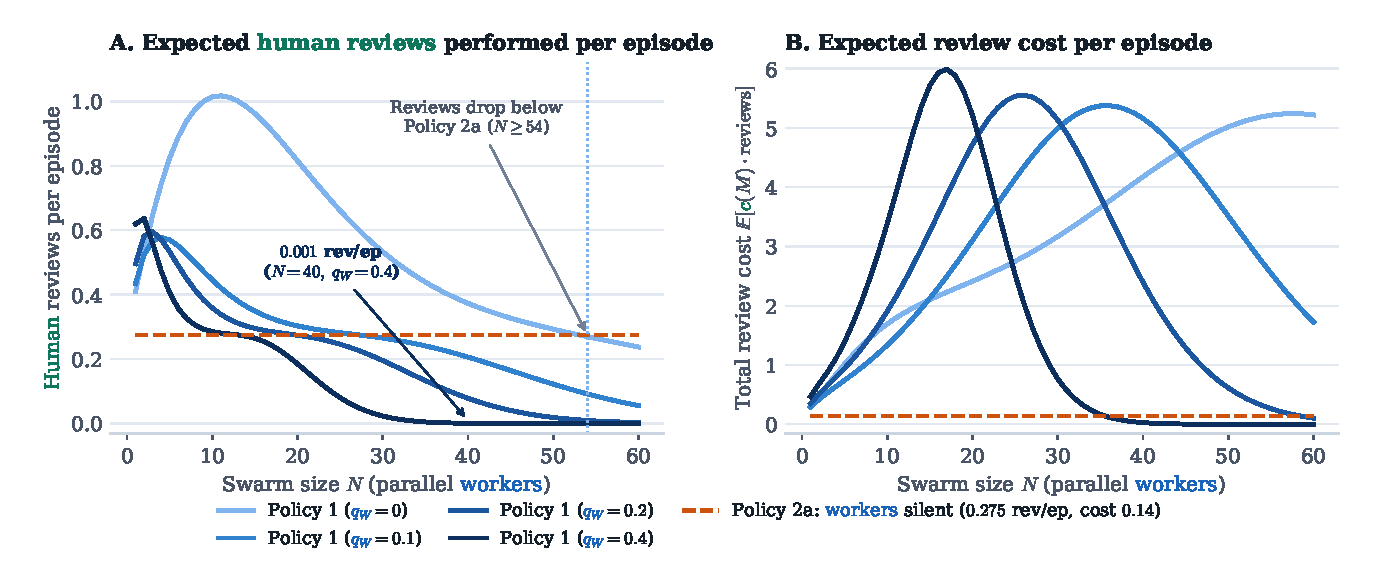
\includegraphics[width=0.86\linewidth]{fig_review_volume.pdf}
  \caption{Non-monotonic \Htxt{human} review volume under convex inbox congestion: (A) expected \Htxt{human} reviews per episode and (B) expected review cost versus swarm size $N$.}
  \label{fig:review_volume}
\end{figure}

\subsection{Permissive Initialization and Single-Asker Trust Traps}
\label{subsec:trust_trap}

Finally, motivated by rising session-level auto-approval among experienced users~\cite{anthropic2026autonomy}, \hyperref[fig:trust_trap]{Figure~\ref{fig:trust_trap}} tests Policy~3 sensitivity to permissive initial \Htxt{human} oversight ($\Hv{p_{H,0}} \ll 1$) at $N = 40, \Wv{q_{W,0}} = 0.4$. Whereas deterministic exact symmetric IPG traps at the \Wtxt{worker}-silent equilibrium only for $\Hv{p_{H,0}} \le 0.0022$, finite-batch noise under sampled $40$-player IPG widens the trust-trap basin up to $\Hv{p_{H,0}} = 0.25$: when \Wtxt{worker} pings are pooled anonymously, even a \emph{single} \Wtxt{worker} drifting to unconditional deferral ($\Wv{h_1} \approx \Wv{q_1} \approx 1$) dilutes the \Wtxt{worker} tier's posterior review value below $\Hv{c}(1)$, making $\trust$ Bayes-optimal for $\Hv{H}$ on all \Wtxt{worker} pings and motivating per-\Wtxt{worker} identity attribution during online calibration.

\begin{figure}[!htbp]
  \centering
  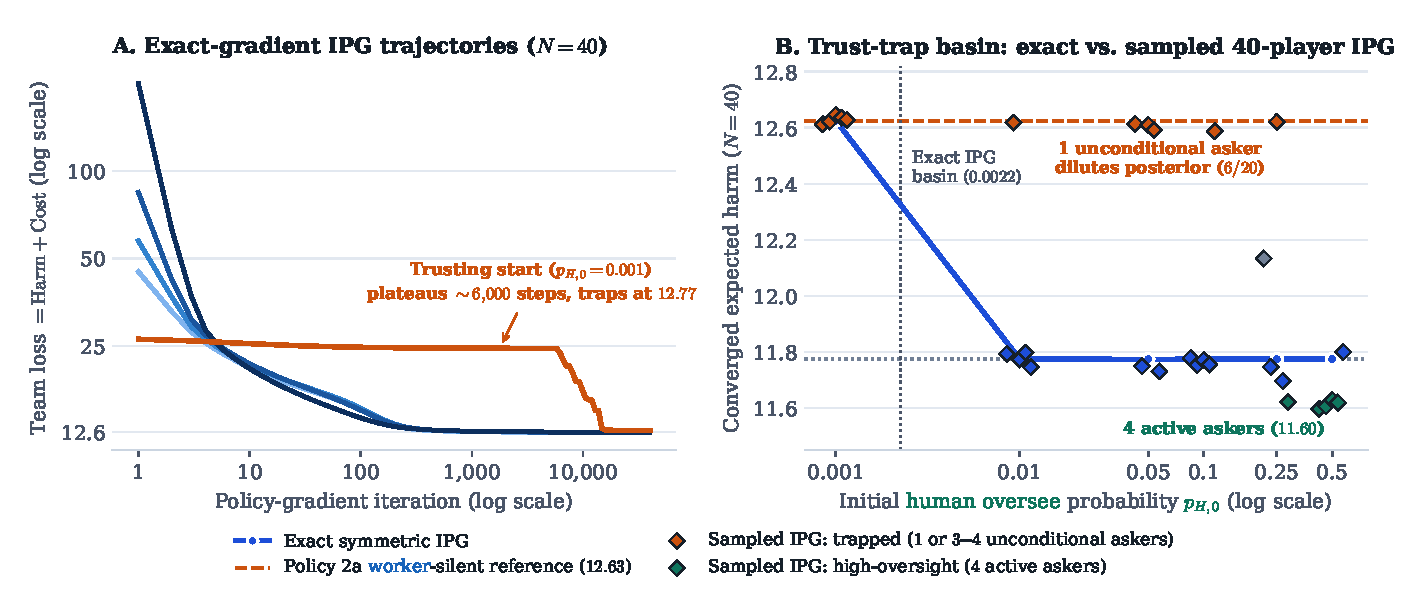
\includegraphics[width=0.88\linewidth]{fig_trust_trap_basin.pdf}
  \caption{Trust-trap basin at $N = 40$ ($\Wv{q_{W,0}} = 0.4$, convex inbox cost): (A) exact symmetric IPG trajectories and (B) exact versus sampled $40$-player IPG across initial \Htxt{human} oversee probabilities $\Hv{p_{H,0}}$.}
  \label{fig:trust_trap}
\end{figure}

\section{Extended Literature Positioning and Architectural Discussion}
\label{app:extra}

\subsection{Extended Related Work and Positioning Matrix}
\label{subsec:related}

\hyperref[tab:lit_matrix]{Table~\ref{tab:lit_matrix}} contrasts our framework against prior and concurrent work across AI oversight, multi-agent systems, queueing, and game-theoretic learning along four threads:
\begin{itemize}
  \setlength{\itemsep}{4pt}
  \item \textbf{Frontier-lab swarm architectures and oversight logs~\cite{anthropic2025research,openai2025agents,kimi2026k25,moonshot2026k25blog,anthropic2026autonomy,paglieri2026swarm,anthropic2026multiagent,greenblatt2024control,lindner2025control,reid2026risks}:}
  Production systems pair a capable \Ftxt{orchestrator} with parallel \Wtxt{workers}: \href{https://www.anthropic.com/research/multi-agent-research-system}{Anthropic's research system}~\cite{anthropic2025research} coordinates a Claude Opus~4 lead over parallel Sonnet~4 \Wtxt{workers}, \href{https://arxiv.org/abs/2602.02276}{Kimi~K2.5}~\cite{kimi2026k25} trains an \Ftxt{orchestrator} over frozen subagents (up to $100$ parallel subagents in Agent Swarm~\cite{moonshot2026k25blog}), \href{https://openai.com/index/new-tools-for-building-agents/}{OpenAI's Agents SDK}~\cite{openai2025agents} provides handoff and guardrail primitives, and evaluation swarms already run $45$--$100$ agents~\cite{anthropic2026multiagent,paglieri2026swarm}. Deployment logs show step-by-step \Htxt{human} review failing to scale uncoordinated: \href{https://www.anthropic.com/research/measuring-agent-autonomy}{Anthropic's autonomy study}~\cite{anthropic2026autonomy} finds \Htxt{human} involvement falling on complex tasks where agents stop to ask more than twice as often as \Htxt{humans} interrupt, AI-control analyses cap synchronous \Htxt{human} audits near $2\%$ of actions to preserve availability across parallel instances~\cite{greenblatt2024control,lindner2025control,reid2026risks}, whistleblowing reports in a $100$-agent proof swarm went unread on an unmonitored organizer endpoint~\cite{paglieri2026swarm}, and same-model \Wtxt{workers} exhibit severe queue contention and correlated behavior~\cite{anthropic2026multiagent}.

  \item \textbf{Oversight games and multi-agent reporting~\cite{overman2026oversight,overman2026conservatism,tong2026contextual,turan2026capacity,mclaughlin2024complementarity,agrawal2026offswitch,wang2026ask,casheekar2026report}:}
  Single-agent Oversight Game extensions study conservative monitor ensembles~\cite{overman2026conservatism}, two-sided private information~\cite{tong2026contextual}, \Htxt{human}--AI complementarity~\cite{mclaughlin2024complementarity}, and fatiguing \Htxt{reviewers}~\cite{turan2026capacity}, while two-agent off-switch games~\cite{agrawal2026offswitch} assume unconstrained \Htxt{human} capacity. Concurrent multi-agent works coordinate clarification requests to one \Htxt{human} via a centralized dynamic program without harm oversight~\cite{wang2026ask} or study PPO reporting under exogenous audits without a capacity-limited \Htxt{human} inbox~\cite{casheekar2026report}; neither studies which subset of identical \Wtxt{workers} may query a congestible \Htxt{human} when \Ftxt{orchestrator} oversight is at stake.

  \item \textbf{Congested learning to defer, priority queues, and robot fan-out~\cite{olsen2004fanout,chien2012queues,dahiya2022restless,hoque2023fleet,costen2024shared,argon2009priority,ouyang2022priorities,lykouris2024congested,alves2024deccaf,zhang2026falcon,saketos2026defer,ancker2017alertfatigue}:}
  Multi-robot supervision allocates scarce \Htxt{operator} attention via centralized scheduling, restless-bandit indices, or bidding~\cite{olsen2004fanout,chien2012queues,dahiya2022restless,hoque2023fleet,costen2024shared}, while learning-to-defer models incorporate queue backlog costs~\cite{lykouris2024congested,saketos2026defer}, batch caps~\cite{alves2024deccaf}, and \Htxt{reviewer} fatigue~\cite{zhang2026falcon,ancker2017alertfatigue}, and queueing theory analyzes noisy priority labels~\cite{argon2009priority,ouyang2022priorities}. \hyperref[prop:noisy_priority]{Propositions~\ref{prop:noisy_priority}}--\hyperref[prop:roster]{\ref{prop:roster}} connect these threads via closed-form swarm crossover laws and pre-inbox roster admission.

  \item \textbf{Symmetry breaking in team games and RL sorting~\cite{marschak1972teams,emmons2022symmetric,duffy2005sorting,whitehead2008elfarol,kleinberg2009multiplicative,hoeffding1956successes,amir2026diversity}:}
  Mixed symmetric local optima in common-payoff team games~\cite{marschak1972teams} are unstable to asymmetric deviations~\cite{emmons2022symmetric}, reinforcement learners in entry, El Farol, and congestion games sort into pure entrants and abstainers~\cite{duffy2005sorting,whitehead2008elfarol,kleinberg2009multiplicative}, Schur-convex objectives reward MARL diversity~\cite{amir2026diversity}, and binary probabilities minimize Bernoulli-sum dispersion~\cite{hoeffding1956successes}. We show that these forces operate in a two-tier oversight game with a co-learning \Htxt{human}, aligning learned \Wtxt{worker} cohorts with the optimal rotating roster.
\end{itemize}

\begin{table}[!htbp]
  \centering
  \caption{Structural comparison with closest prior and concurrent literature ($\checkmark$ = modeled; $\sim$ = partial; --- = absent).}
  \label{tab:lit_matrix}
  \resizebox{\linewidth}{!}{%
  \begin{tabular}{@{}lccccccc@{}}
    \toprule
    Prior / Concurrent Work & Multi-AI, $1$ $\Hv{H}$ & $\Hv{H}$ Capacity & \Wtxt{Worker} $\ask$ & Eq.\ / Learn & \Wtxt{Worker} Sort & $\Fv{F}$ vs.\ $\Wv{W}$ Tiers & Harm Ovs. \\
    \midrule
    Overman \& Bayati~\cite{overman2026oversight}            & --- & $\sim$ (cost) & $\checkmark$ & $\checkmark$ & --- & --- & $\checkmark$ \\
    Agrawal et al.~\cite{agrawal2026offswitch}               & $\checkmark$ ($2$-agent) & --- & $\checkmark$ & $\sim$ (pure) & --- & --- & $\checkmark$ \\
    Turan~\cite{turan2026capacity}; FALCON~\cite{zhang2026falcon}; DeCCaF~\cite{alves2024deccaf} & --- & $\checkmark$ & --- & --- & --- & --- & $\sim$ \\
    Lykouris \& Weng~\cite{lykouris2024congested}; Saketos et al.~\cite{saketos2026defer} & --- & $\checkmark$ & --- & $\sim$ ($1$ AI) & --- & --- & --- \\
    Greenblatt et al.~\cite{greenblatt2024control}; Lindner et al.~\cite{lindner2025control} & $\checkmark$ & $\checkmark$ ($2\%$) & --- (monitor) & --- & --- & --- & $\checkmark$ \\
    Paglieri et al.~\cite{paglieri2026swarm}                 & $\checkmark$ & --- (unread) & $\checkmark$ & --- & $\sim$ (empirical) & --- & $\checkmark$ \\
    Costen et al.~\cite{costen2024shared}; Dahiya et al.~\cite{dahiya2022restless} & $\checkmark$ & $\checkmark$ & $\sim$ (bids) & --- & --- & --- & --- \\
    Wang, Liu, \& Wang~\cite{wang2026ask}                    & $\checkmark$ & $\checkmark$ & --- (central) & --- & --- & $\sim$ (weights) & --- \\
    Casheekar \& Tangirala~\cite{casheekar2026report}        & --- (audit) & --- & $\checkmark$ & $\checkmark$ & $\sim$ (groups) & --- & $\checkmark$ \\
    Emmons et al.~\cite{emmons2022symmetric}; Duffy \& Hopkins~\cite{duffy2005sorting} & --- & $\sim$ (entry) & $\checkmark$ & $\checkmark$ & $\checkmark$ & --- & --- \\
    \midrule
    \textbf{This work}                                       & $\checkmark$ & $\checkmark$ & $\checkmark$ & $\checkmark$ & $\checkmark$ & $\checkmark$ & $\checkmark$ \\
    \bottomrule
  \end{tabular}}
\end{table}

\subsection{Architectural Discussion: Parameter Sharing and Modeling Scope}
\label{subsec:discussion}

\begin{itemize}
  \setlength{\itemsep}{4pt}
  \item \textbf{Parameter sharing in deployed LLM swarms versus independent-parameter IPG:}
  Production swarms typically instantiate \Wtxt{workers} as copies of one frozen weight vector ($\Wv{\sigma_i} \equiv \Wv{\sigma_W}$)~\cite{anthropic2025research,kimi2026k25,paglieri2026swarm}. Without agent-specific role conditioning, shared-parameter \Wtxt{workers} remain on the symmetric subspace ($\Wv{h_1} = \dots = \Wv{h_N}$, matching Policy~3's exact symmetric IPG column in \hyperref[fig:specialization]{Figure~\ref{fig:specialization}} rather than sampled $N$-player IPG; cf.~\cite{casheekar2026report}). Accordingly, our \textbf{fixed-size rotating roster} serves as the direct zero-training policy for weight-sharing deployments, while independent-parameter IPG confirms game-theoretically that decentralized optimization selects the same binary cohort structure.

  \item \textbf{Modeling scope and prospective calibration:}
  Asymmetry $\Fv{L_F} \gg \Wv{L_W}$ reflects architectural authority---$\Fv{F}$ synthesizes subagent outputs and commits external actions~\cite{anthropic2025research,kimi2026k25}, so unreviewed \Ftxt{orchestrator} errors corrupt the final outcome rather than averaging across subtasks---while convex cost $\Hv{c}(m)$, hard cap $\Hv{K}$, and exponential fatigue $\Hv{\xi}(m)$ provide tractable stylized forms ahead of extensions to cross-episode backlogs~\cite{lykouris2024congested,saketos2026defer}, non-monotonic clinical alert overrides~\cite{ancker2017alertfatigue}, and correlated \Wtxt{worker} failures~\cite{anthropic2026multiagent}. Prior to the final report, a lightweight pass on $20$--$30$ \href{https://arxiv.org/abs/2309.15817}{ToolEmu}~\cite{ruan2024toolemu} scenarios~\cite{overman2026oversight} can empirically anchor $(\Wv{p_W}, \Wv{q_W}, \Hv{\varepsilon})$ on our phase diagrams. \emph{GenAI disclosure:} Claude and Gemini assisted with literature verification, simulation scripting, and typesetting; all derivations, numerical checks, and claims were independently audited by the authors.
\end{itemize}

\end{document}
